\documentclass{IEEEtran}

\usepackage{amsmath}
\usepackage{amssymb}
\usepackage{amsfonts}

\ifCLASSINFOpdf
   \usepackage[pdftex]{graphicx}
\else
   \usepackage[dvips]{graphicx}
\fi

\ifCLASSOPTIONcompsoc
  \usepackage[caption=false, font=normalsize, labelfont=sf, textfont=sf]{subfig}
\else
  \usepackage[caption=false, font=footnotesize]{subfig}
\fi

\usepackage{textcomp}
\usepackage{nicefrac}
\usepackage{siunitx}
\usepackage{fancyref}

\usepackage[style=ieee, doi=false, isbn=false, url=false, maxbibnames=1, minbibnames=1, maxcitenames=1, mincitenames=1, backend=biber, defernumbers=false]{biblatex}
\addbibresource{./references.bib}

\AtEveryBibitem{\clearfield{month}}
\AtEveryBibitem{\clearfield{day}}
\AtEveryBibitem{\clearfield{volume}}
\AtEveryBibitem{\clearfield{issue}}
\AtEveryBibitem{\clearfield{pages}}
\AtEveryBibitem{\clearfield{number}}
\AtEveryBibitem{\clearfield{title}}
\AtEveryBibitem{\clearfield{isbn}}
\AtEveryBibitem{\clearfield{keywords}}
\AtEveryBibitem{\clearfield{issn}}
\AtEveryBibitem{\clearfield{journal}}

\usepackage[activate={true, nocompatibility}, final, tracking=true, kerning=true, spacing=true, factor=1100, stretch=10, shrink=10]{microtype}
\linespread{0.9}

\usepackage{glossaries}

\newacronym{AI}{AI}{Artificial Intelligence}
\newacronym{AE}{AE}{Auto-Encoder}
\newacronym{AC}{AC}{Attenuation Correction}
\newacronym{ALS}{ALS}{Amyotrophic Lateral Sclerosis}
\newacronym{GPU}{GPU}{Graphics Processing Unit}
\newacronym{FDG}{FDG}{fluorodeoxyglucose}
\newacronym{AIF}{AIF}{Arterial Input Function}
\newacronym{AUC}{AUC}{Area Under the Curve}
\newacronym{cLBP}{cLBP}{chronic Low Back Pain}
\newacronym{CV}{nCV}{Normalised Coefficient of Variance}
\newacronym{MSE}{MSE}{Mean Squared Error}
\newacronym{MR}{MR}{Magnetic Resonance}
\newacronym{PBR28}{[$^{11}$C]-PBR$28$}{[$^{11}$C]-Peripheral Benzodiazepine Receptor}
\newacronym{MNI}{MNI}{Montreal Neurological Institute}
\newacronym{FWHM}{FWHM}{Full Width Half Maximum}
\newacronym{HC}{HC}{Healthy Control}
\newacronym{HAB}{HAB}{High Affinity Binder}
\newacronym{MAB}{MAB}{Mixed Affinity Binder}
\newacronym{PT}{PT}{Patient}
\newacronym{HPLC}{HPLC}{High Performance Liquid Chromatography}
\newacronym{IDIF}{IDIF}{Image Derived Input Function}
\newacronym{LL}{LL}{Log-Likelihood}
\newacronym{LSTM}{LSTM}{Long Short Term Memory}
\newacronym{KOA}{KOA}{Knee Osteo-Arthritis}
\newacronym{MAE}{MAE}{Mean Absolute Error}
\newacronym{ML}{ML}{Machine Learning}
\newacronym{NN}{NN}{Neural Network}
\newacronym{SUV}{SUV}{Standardised Uptake Value}
\newacronym{TAC}{TAC}{Time Activity Curve}
\newacronym{OSEM}{OSEM}{Ordered Subset Expectation Maximisation}
\newacronym{PET}{PET}{Positron Emission Tomography}
\newacronym{ROI}{ROI}{Region Of Interest}
\newacronym{RMSE}{RMSE}{Root Mean Squared Error}
\newacronym{TSPO}{TSPO}{Translocator Protein 18 kDa}
\newacronym{TCM}{TCM}{Tissue Compartment Model}
\newacronym{SNR}{SNR}{Signal to Noise Ratio}
\newacronym{mCi}{mCi}{Millicurie}
\newacronym{VT}{V$_{\mathrm{T}}$}{Volume of Distribution}
\newacronym{IF}{IF}{Input Function}
\newacronym{NLP}{NLP}{Natural Language Processing}

\begin{document}
    \title{
        \vspace{-0.75cm}
        
        A Bayesian Neural Network-Based Method for the Extraction of a Metabolite Corrected Arterial Input Function from Dynamic [$^{11}$C]PBR28 PET 
    }
    
    \author{
        \vspace{-0.25cm}
        
        Alexander~C.~Whitehead$^{*}$~\IEEEmembership{Student~Member,~IEEE},
        Ludovica~Brusaferri$^{*}$,
        Lucia~Maccioni,
        Matteo~Ferrante,
        Marianna~Inglese,
        Zeynab~Alshelh,
        Mattia~Veronese,
        Nicola~Toschi,
        Jodi~Gilman,
        Kris~Thielemans,
        and~Marco~L.~Loggia
    
        \vspace{-0.75cm}
    
        \thanks{
            \scriptsize
            This work was funded by GE Healthcare, the NIHR UCLH Biomedical Research Centre, the UCL EPSRC Centre for Doctoral Training in Intelligent, Integrated Imaging in Healthcare(i4health) grant(EP/L016478/1), the Open Source Imaging Consortium(OSIC), the NIH grants R01-NS094306-01A1, R01-NS095937-01A1 and R01-DA047088-01, the Italian Ministry of University and Research(MUR), National Recovery and Resilience Plan(NRRP), project MNESYS(PE0000006)(to NT)–A Multiscale integrated approach to the study of the nervous system in health and disease(DN.1553 11.10.2022), National Center for HPC, BIG DATA AND QUANTUM COMPUTING(Project no.CN00000013CN1), the PNRR National Grant DIGITAL LIFELONG PREVENTION(Project no PNC0000002DARE), and by Wellcome Trust Digital Award(no.215747/Z/19/Z).
        }
        \thanks{
            \scriptsize
            Alexander~C.~Whitehead is with the Department of Computer Science, University College London, London, UK. Ludovica~Brusaferri, Zeynab~Alshelh, Jodi~Gilman, Nicola~Toschi, and Marco~L.~Loggia are with Athinoula A. Martinos Center for Biomedical Imaging, Harvard Medical School, Boston, MA, US. Lucia~Maccioni and Mattia~Veronese are with the Department of Information Engineering, University of Padua, Padua, Italy and Neuroimaging Department, IoPPN, King’s College London, London, UK. Matteo~Ferrante, Marianna~Inglese, and Nicola~Toschi are with the Department of Biomedicine and Prevention, University of Rome Tor Vergata, Rome, Italy.
        }
    }
    
    \pagestyle{plain}
    \pagenumbering{gobble}
    
    \maketitle
    
    \begin{abstract}
        In Positron Emission Tomography (PET), arterial sampling and metabolite correction are prerequisites for the gold-standard measurement of values like the volume of distribution ($\mathrm{V_T}$), often necessary for the full quantification of radioligand binding. However, the invasiveness and technical demands of these procedures limit their application in both research and clinical PET studies. Machine learning approaches have been explored to predict $\mathrm{V_T}$ from PET images, but their integration in clinical routine is limited by their lack of transparency or thorough evaluation. Here we propose a Bayesian Neural Network to estimate the arterial input function (AIF), while also outputting its prediction uncertainty, 1) directly from the entire dynamic PET images (NN-AEIF), 2) from an image-derived input function (IDIF) (NN-IDIF) and, as a sensitivity measure, 3) from the un-corrected plasma curve (NN-AIF). All methods, applied on [$^{11}$C]PBR28 PET data, were compared to the metabolite-corrected AIF in terms of $\mathrm{V_T}$, and the prediction uncertainty was assessed in terms of normalised coefficient of variance (nCV). Overall, both NN-AEIF and NN-AIF were able to accurately predict $\mathrm{V_T}$, outperforming the other methods, with NN-AEIF showing the lowest nCV.
    \end{abstract}
    
    % \begin{IEEEkeywords}
      %   Arterial Input Function Estimation, Signal Extraction, Dynamic PET, Machine Learning, Bayesian Neural Networks
     % \end{IEEEkeywords}
    
    \vspace{-0.5cm}

\section{Introduction} \label{sec:introduction}\vspace{-0.3cm}\vspace{0.2cm}
    \IEEEPARstart{T}{he} \gls{VT} estimated with an \gls{AIF} is utilised for quantification of many \gls{PET} tracers, including \gls{PBR28}. This, however, requires the concurrent measurement of the concentrations of unchanged radioligand in arterial plasma. Although insertion of an arterial catheter rarely results in clinically relevant adverse events, it is an invasive and laborious procedure. 
    
    \gls{IDIF} represents a promising alternative to arterial sampling~\cite{Zanotti-Fregonara2011}. However, its applicability in clinical research is hampered by several factors including the inaccuracy in the estimation of both shape and amplitude of the \gls{IF}; moreover \gls{IDIF} does not allow for radio-metabolites quantification~\cite{Sari2018Non-invasive11C-SB201745}. The application of \gls{ML} is expected to improve the accuracy of predicting the \gls{AIF} from \gls{PET} images~\cite{Kuttner2020, Ferrante2022PhysicallyImaging}. While these methods have shown promising results, the vast majority of these approaches have been developed for \gls{PET} tracers that do not produce radio-metabolites. Furthermore, even if the developed model shows sufficient prediction accuracy for unseen data, its applicability in the clinical setting remains questionable because of a lack of transparency or thorough evaluation~\cite{Salahuddin2022TransparencyMethods}. Bayesian networks offer the significant advantage of making probabilistic predictions based on available evidence. Specifically, a Bayesian network would output uncertainty estimates in addition to the model prediction. For this reason, they have the potential to overcome the key barrier to the responsible adoption of \gls{AI} in clinical practice~\cite{Prabhudesai2023LoweringAI}. 
    
    Here, we propose a Bayesian \gls{NN}-based method for predicting a metabolite corrected \gls{AIF}, while allowing for the estimation of uncertainty of the model's output.% Specifically for the \gls{AE}, although also present in the other networks, we try to enforce the low dimensional representation of the input data as disentangled and continuous. Furthermore, the network does not predict a single signal for each input; rather, it predicts a probability density function of potential signals, which allows for the estimation of uncertainty of the model's output.

    \vspace{-0.5cm}

\section{Methods} \label{sec:methods}     
    \subsection{Data Acquisition and Processing}\label{sec:dataproc}
        Dynamic \gls{PBR28} \gls{PET}/\gls{MR} images from $52$ individuals (Age: $55 \pm 16$ years; Sex: $27$ Male, $25$ Female; Genotype: $32$ \glspl{HAB}, $20$ \glspl{MAB}; Clinical population: $12$ Healthy Controls, $40$ Chronic Pain patients; Injected Dose: $14.16 \pm 1.3$ \glspl{mCi}) were acquired on a Siemens Biograph mMR whole-body tomograph for a time-period of $0$-$90$ minutes post-injection. Data were pooled for multiple protocols (approved by the Partners Healthcare/Mass General Brigham Institutional Review Board) and reconstructed as in \cite{Brusaferri2022ThePandemic}. All subjects had a radial artery catheter placed during the scan. Uncorrected plasma curves from blood samples were interpolated and metabolite-corrected to obtain the \gls{AIF}. To further validate the proposed method, \gls{IDIF} was calculated by segmenting the arterial carotid siphons using intensity thresholding of early dynamic \gls{PET} frames. Data were split using ten-fold cross-validation, ensuring maximum within-variance and minimum between-variance in the training and testing sets.
        
        % All subjects received a radial artery catheter at the time of the scan. Uncorrected plasma curves from the blood samples were interpolated and metabolite-corrected to obtain the \gls{AIF}. Uncorrected plasma curves were obtained from raw blood samples using linear fitting. In $16$ subjects, arterial blood processing was performed using a HyperSep C$18$ solid extraction cartridge to separation of radio-metabolites; in $36$ subjects, \gls{HPLC} for separation of radio-metabolites from parent radiotracer was used instead. Hill-fitted parent fractions were applied to the raw data and a radio-metabolite-corrected \gls{AIF} was obtained for each subject. Previous cross-validation confirmed reliability of both pipelines allowing for the combination of both data-sets to increase statistical power of the study~\cite{Brusaferri2022ThePandemic}. 
        
        % For validation purposes, \gls{IDIF} was also calculated by segmenting the arterial carotid siphons via intensity thresholding of early  dynamic \gls{PET} frames. Data were split following ten-fold cross validation. The split was specifically designated to maximise the within-variance while minimising the between-variance in training and testing sets.

    \vspace{-0.5cm}
    
    \subsection{Neural Network Design}\label{sec:NNDesign}
        The method is comprised of three independent \glspl{NN}: \gls{NN}$_1$ seeks to reduce the dimentionality of the input data (due to computational requirements) and extract the most relevant features. \gls{NN}$_2$ aims to extract a non-metabolite corrected signal from the low-dimensional representation output by the first network. \gls{NN}$_3$ metabolite corrects and reshapes/rescales the non-metabolite corrected signal. 
        
        % All models use a novel activation function, defined as $PSoftplus = \log\big(\mathrm{e}^{x} + \alpha^2 \big)$, where $x$ is the output from the previous layer and $\alpha$ is a learnt parameter which is initialised as $\alpha = 0$.  This activation function was designed as a fully differentiable drop-in replacement for \textit{PReLU} \cite{Ciuparu2020Soft++Architectures}. The initial value of $\alpha$ is selected such that the activation is initially linear (thus making the model easier to train at early iterations) and becomes non-linear as training progresses.
        % https://www.sciencedirect.com/science/article/pii/S0925231219317163

        % In order to try to enforce disentanglement and continuity of this layer, a regularisation term to enforce the orthogonality of its output was used. To promote stability of the optimisation, a regularisation term which compares the area under the curve of the prediction and true signals was used in each \gls{NN}. Common to all \glspl{NN}, each model was optimised using AdaBelief~\cite{Zhuang2020AdaBeliefGradients} with the warm-up proportion equivalent to one-tenth of the total number of epochs, after which it does not decrease. Weight decay was used to regularise against large weights. %Each model was trained initially using \gls{RMSE}, where the mean output of the model is penalised against the expected value and the standard deviation output of the model is encouraged to be close to $1$. Subsequently, a second training regime was used where the negative \gls{LL} function is used to fine-tune the parameters. Gradient accumulation was used to allow for only one data-point to be loaded onto the \gls{GPU} at any one time and for any arbitrary batch-size to be used. The batch size starts at two and increases to the size of total number of data points, where the batch size doubles as the current epoch number quadruples.

        \subsubsection{\gls{NN}$_1$ \gls{AE}} \label{sec:NN1}
            This network features three blocks, the downsampling block, the latent layer, and the upsampling block. The first block comprises three convolutions; the latent block is flanked on either side by two convolutions, with a variational latent layer in the middle. The upsampling block consists of a transposed convolution and two standard convolutions. Here, two downsampling and two upsampling blocks here used. The number of filters doubled or halved at each block respectively.
            
            The input to the network is the dynamic \gls{PET} images. Both the mean and standard deviation of the latent layer and the final layer are output from the model and passed onto \gls{NN}$_2$. Both input and target data were standardised separately, based on parameters obtained from the training set. Each time frame was treated as an independent training example.

            % The target images were smoothed using a Gaussian filter with a \gls{FWHM} equal to three times the voxel size in each dimension. All images were padded such that the size of each dimension was equal to the next larger power of two. Both input and target images were standardised separately, based on parameters obtained from the training set.

        \subsubsection{\gls{NN}$_2$ Signal Extractor} \label{sec:NN2}
            This network consists of two blocks, the downsampling block and the fully connected block. The downsampling block follows the same structure as in \gls{NN}$_1$. The fully connected block consists solely of one fully connected layer. All time frames were used simultaneously, where the same convolutions are applied independently on each time frame before global average pooling and flattening. After flattening the clinical features were concatenated with the flattened output. Here, four downsampling blocks and eight fully connected blocks were used. The number of filters doubled and the number of units halved at each block respectively.

            % Each element of the clinical features was either standardised or encoded using one hot encoding depending on the nature of the feature. Because the autoencoder outputs both a mean and a standard deviation values were sampled at the input of the network using the same \textit{reparametrisation-trick} as for a variational autoencoder.
            
        \subsubsection{\gls{NN}$_3$ Metabolite Correction and Reshaping} \label{sec:NN3}
            This network contains solely fully connected layers. If the network is to metabolite-correct a signal (e.g. from \gls{AIF} or \gls{IDIF}), it takes that signal as input together with the clinical/demographic features (age, sex, genotype, injected dose, clinical population).  If the network is instead to correct a signal obtained with \gls{NN}$_2$, both the mean and the standard deviation of the uncorrected signal are input to \gls{NN}$_3$, in addition to the latent layer from \gls{NN}$_2$.

    \vspace{-0.5cm}
    
    \subsection{Evaluation}\label{sec:evaluation}        
        The model was sampled $32$ times resulting in multiple realisations of the estimated signal. Then, $V_{\mathrm{T}} \in \mathbb{R}^{r \times s \times b}$ were computed via the Logan graphical method, where $r$ is the number of \glspl{ROI} ($r = 69$), $s$ is the number of subjects ($s = 5$) and $b$ is the number of model samples ($b = 32$). For both \gls{AIF} and \gls{IDIF}, $b=1$. For the \gls{NN}-based methods, \gls{VT} were computed for each model realisation and then used to calculate the mean \gls{VT} and its standard deviation. Moreover, the \gls{CV} was defined as $\mathrm{nCV} = \mathrm{std} (Pred \; V_{\mathrm{T}}) / True \; V_{\mathrm{T}}$ with $\mathrm{nCV} \in \mathbb{R}^{r \times s}$, where $V_{\mathrm{T}}$ is computed from the measured \gls{AIF}. For each candidate signal, correlation analyses were performed on the \gls{VT} values (computed for all the \glspl{ROI} and for all the subjects in the test-set) to the ones obtained with the ground truth signal (\textbf{TRUE-\gls{AIF}}, see~\Fref{sec:dataproc}). To measure the accuracy of the prediction, the angle between the regression- and the identity-line was also computed, defined as $\theta = 45 - \arctan(m)*180/\pi$, with $m$ being the slope of the regression-line. Furthermore, \glspl{CV} were averaged across \glspl{ROI} for each subject of the test-set and compared via a paired t-test for each of the three \gls{NN}-based methods.
       
        \subsubsection*{Candidate Signals} \label{sec:candidates}
            \begin{itemize}
                \item \textbf{\gls{IDIF}} - generated as in~\Fref{sec:dataproc}.
                
                \item \textbf{\gls{NN}-\gls{IDIF}} - metabolite-corrected \gls{IF} obtained from \gls{IDIF} input to \gls{NN}$_3$.
                
                \item \textbf{\gls{NN}-\gls{AIF}} - metabolite-corrected \gls{AIF} obtained from (uncorrected) arterial plasma input to \gls{NN}$_3$.
                
                \item \textbf{\gls{NN}-\gls{AE}\gls{IF}} - metabolite-corrected \gls{IF} obtained from dynamic \gls{PET} images input to \gls{NN}$_{1,2,3}$.
            \end{itemize}

    \vspace{-0.5cm}

\section{Results} \label{sec:results}
    \begin{figure}
        \vspace{-0.5cm}
        
        \centering
        
        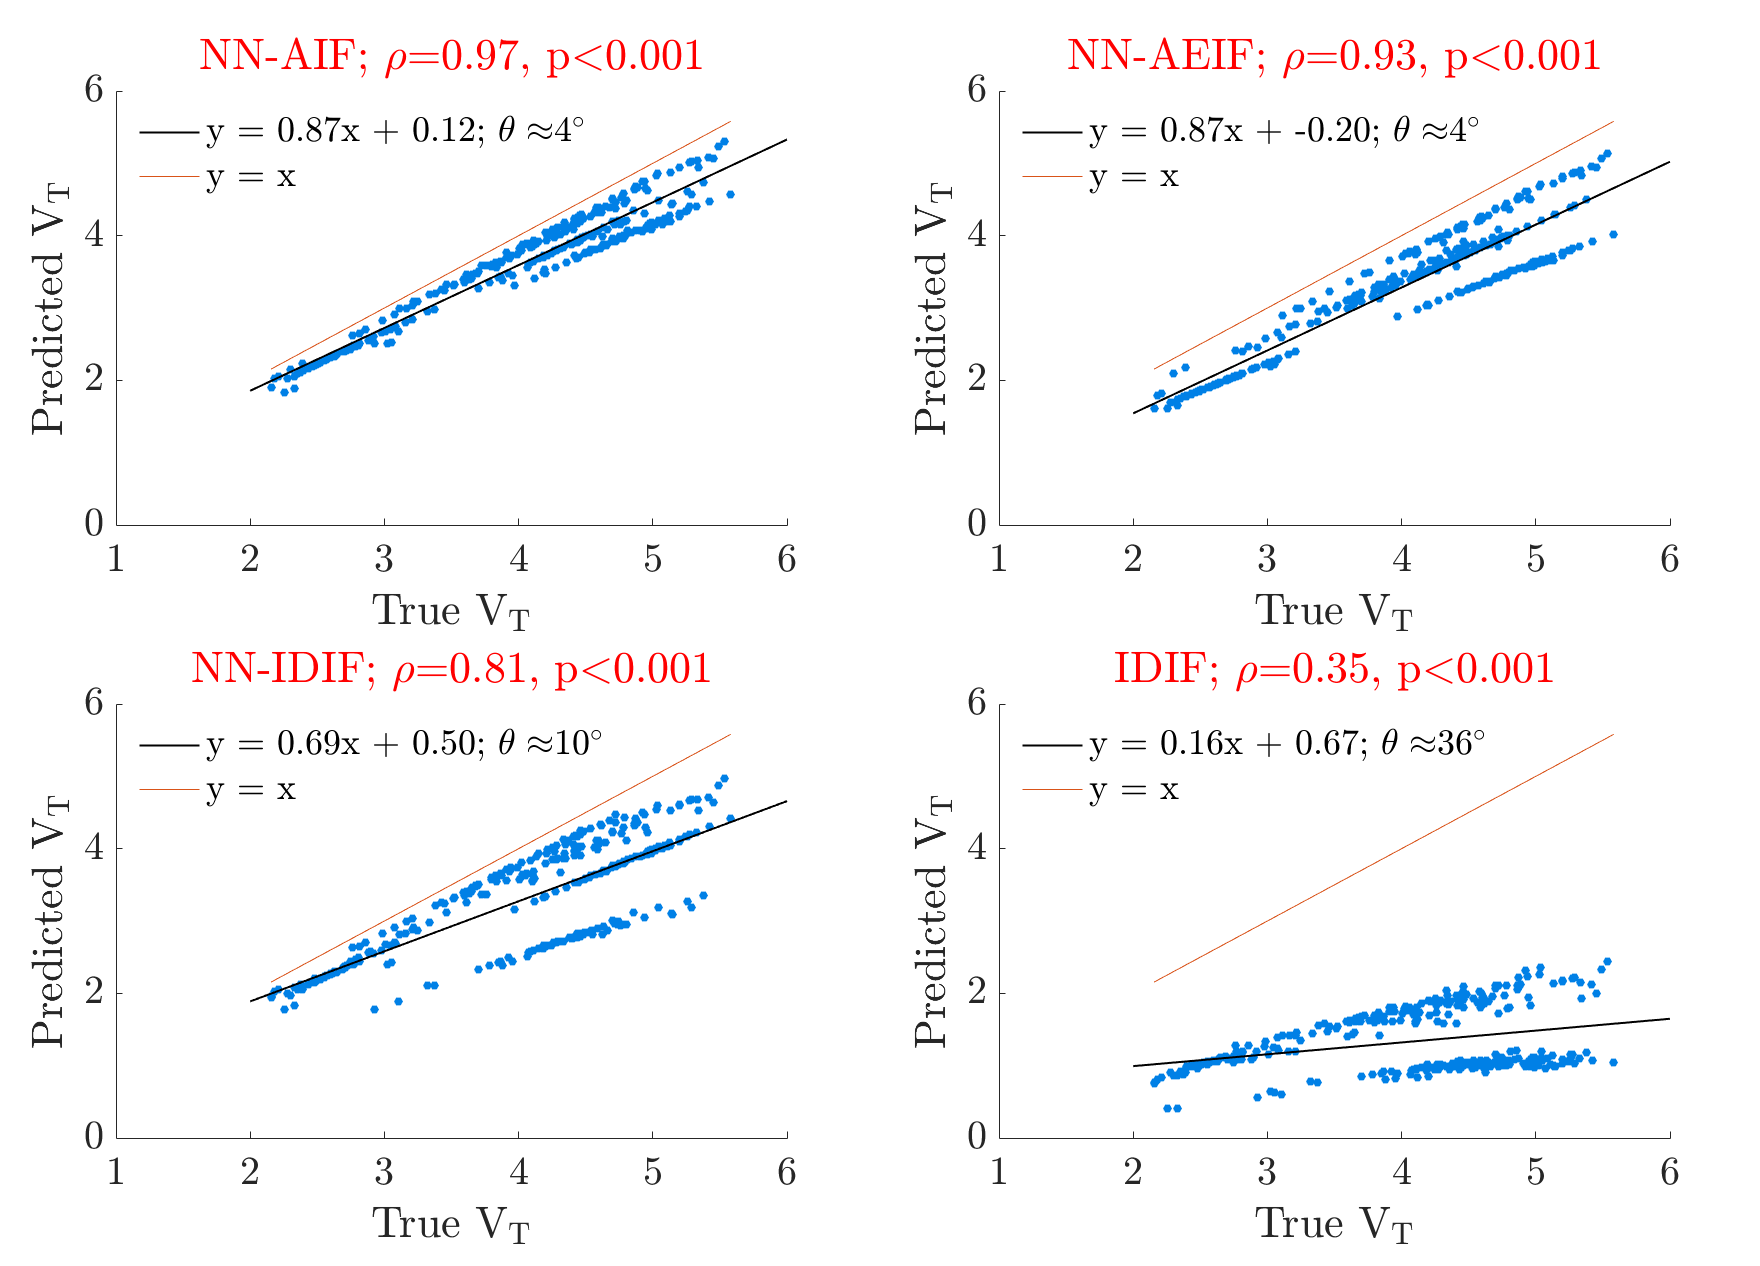
\includegraphics[width=1.0\linewidth]{Figures/correlation.png}
        
        \vspace{-0.25cm}
        
        \captionsetup{singlelinecheck=false, justification=centering}
        \caption{
            \scriptsize
            Predicted $V_{\mathrm{T}} \in \mathbb{R}^{r \times s}$ in the test-set subjects, with $r = 69$ and $s=5$ estimated with the four candidate signals, correlated to the True \gls{VT} (obtained with TRUE-\gls{AIF}). Please note that for the \gls{NN}-based methods, the displayed \glspl{VT} was averaged over all realisations.
        }
        
        \label{fig:correlation}
        
       \vspace{-0.5cm}
   \end{figure}

    
   \Fref{fig:correlation} reports the correlation analyses between the predicted \gls{VT} values (obtained by the four candidate methods) and the true \gls{VT} values. For all methods, predicted \gls{VT} values positively correlate with true \gls{VT} values, with \gls{NN}-\gls{AIF} and \gls{IDIF} showing the highest and the lowest Pearson correlation coefficient ($\rho$), as well as the smallest and largest angular distance to the identity line, respectively: $\rho = 0.97 \; \& \;  \theta \approx 4^{\circ}$ vs $\rho = 0.35 \; \&  \; \theta \approx 36^{\circ}$. Overall, \gls{NN}-\gls{AE}\gls{IF} outperformed \gls{NN}-\gls{IDIF} in terms of Pearson correlation coefficient and angular distance: $\rho = 0.93 \; \& \; \theta  \approx 4^{\circ}$ vs $\rho = 0.81 \; \&  \; \theta \approx 10^{\circ}$. With regard to the variance analysis, \gls{NN}-\gls{AE}\gls{IF} outperforms both \gls{NN}-\gls{AIF} and \gls{NN}-\gls{IDIF}, showing the lowest \gls{CV}, while \gls{NN}-\gls{AIF} and \gls{NN}-\gls{IDIF} do not differ in terms of \gls{CV} values (p$>0.05$).

    \vspace{-0.3cm}

\section{Discussion and Conclusion} \label{sec:discussion}
    This work presents an innovative Bayesian \gls{NN}-based approach for estimating the \gls{AIF} from dynamic \gls{PET} images and clinical variables. This approach shares similarities with previous methods developed for \gls{PET} tracers that do not produce radio-metabolites, such as [$^{18}$F]\gls{FDG}. In this study, additional efforts were devoted to address \gls{PBR28} radio-metabolite correction. One of the main advantages of the proposed method is that it provides a measure of confidence in the generated signal for unseen data. Additionally, the method's modular design allows each part to be used independently. For example, in this work, metabolite correction was applied to a signal generated by a more traditional method (\gls{IDIF}). 
    
    The four candidate signals were compared to the gold standard TRUE-\gls{AIF}, obtained from arterial blood sampling and metabolite correction. Overall, \gls{NN}-\gls{AE}\gls{IF} demonstrated comparable performance in terms of correlation and bias to \gls{NN}-\gls{AIF}, with the lowest variance of the estimated \gls{VT}, as measured by the \gls{CV}. This improved performance can potentially be explained by the larger amount of input data and the consequently more complex model with additional parameters. Interestingly, the \gls{NN}-\gls{IDIF} method was able to improve on the traditional \gls{IDIF} approach, as evidenced by a higher correlation coefficient and a lower angular distance from the identity line.
    
    The proposed approach has some limitations, including the small training size, which hindered the assessment of the prediction accuracy within subsets of clinical populations in the test-set (i.e., patients vs healthy controls). In the future, the accuracy of the model could be improved through the inclusion of an attention layer either before or after the latent layer of the \gls{AE}, validated through the use of an ablation study. As well as the replacement of the fully connected layers with a transformer based approach.

    
    \vspace{-0.5cm}
    
    \AtNextBibliography{
        \scriptsize
    }
    \printbibliography
\end{document}
